\documentclass[manuscript,review]{acmart}

\usepackage{lipsum}
\usepackage{subfiles}
\usepackage{graphicx,wrapfig,lipsum}
\usepackage{todonotes}
\usepackage{listings} % Für Code-Darstellung
\usepackage{xcolor}   % Für Farben im Code

% SQL-Formatierung definieren
\lstset{
    language=SQL,                % Sprache auf SQL setzen
    basicstyle=\ttfamily\small,  % Schriftart und -größe
    keywordstyle=\color{blue},   % Schlüsselwörter blau
    stringstyle=\color{red},     % Strings rot
    commentstyle=\color{green},  % Kommentare grün
    showstringspaces=false,      % Keine Leerzeichen in Strings anzeigen
    frame=single,                % Rahmen um den Code
    breaklines=true,             % Zeilenumbruch erlauben
    numbers=left,                % Zeilennummern links
    numberstyle=\tiny\color{gray}% Stil der Zeilennummern
}

%%
%% \BibTeX command to typeset BibTeX logo in the docs
\AtBeginDocument{%
  \providecommand\BibTeX{{%
    Bib\TeX}}}

%% Rights management information.  This information is sent to you
%% when you complete the rights form.  These commands have SAMPLE
%% values in them; it is your responsibility as an author to replace
%% the commands and values with those provided to you when you
%% complete the rights form.
\setcopyright{rightsretained}
\copyrightyear{2025}
\acmYear{2025}
\acmDOI{}
%\acmISBN{978-1-4503-XXXX-X/18/06}
\acmConference[Human-Computer Interaction \& Artificial Intelligence]{Final Project for the HIC Module at the Bergische Universität Wuppertal}{October 7--February 28, 2025}{Wuppertal, Germany}
\acmBooktitle{Final Project for the HIC Module at the Bergische Universität Wuppertal(Human-Computer Interaction \& Artificial Intelligence), October 7--February 28, 2025, Wuppertal, Germany}


%%
%% Submission ID.
%% Use this when submitting an article to a sponsored event. You'll
%% receive a unique submission ID from the organizers
%% of the event, and this ID should be used as the parameter to this command.
%%\acmSubmissionID{123-A56-BU3}

%%
%% For managing citations, it is recommended to use bibliography
%% files in BibTeX format.
%%
%% You can then either use BibTeX with the ACM-Reference-Format style,
%% or BibLaTeX with the acmnumeric or acmauthoryear sytles, that include
%% support for advanced citation of software artefact from the
%% biblatex-software package, also separately available on CTAN.
%%
%% Look at the sample-*-biblatex.tex files for templates showcasing
%% the biblatex styles.
%%

%%
%% The majority of ACM publications use numbered citations and
%% references.  The command \citestyle{authoryear} switches to the
%% "author year" style.
%%
%% If you are preparing content for an event
%% sponsored by ACM SIGGRAPH, you must use the "author year" style of
%% citations and references.
%% Uncommenting
%% the next command will enable that style.
%%\citestyle{acmauthoryear}


%%
%% end of the preamble, start of the body of the document source.
\begin{document}

%%
%% The "title" command has an optional parameter,
%% allowing the author to define a "short title" to be used in page headers.
\title{Natural Language Meets Database:
System Transparency and User
Understanding in NL-to-SQL
Translation}
%\renewcommand{\shortauthors}{Trovato et al.}
\author{Parssa Jashnieh}
\author{Thivyan Sivananthan}
\author{Jacob Ortenberg}
\address{Bergische Universität Wuppertal}

%%
%% The abstract is a short summary of the work to be presented in the
%% article.
\subfile{sections/abstract/Abstract.tex}


%%
%% The code below is generated by the tool at http://dl.acm.org/ccs.cfm.
%% Please copy and paste the code instead of the example below.
%%
\begin{CCSXML}
  <ccs2012>
     <concept>
         <concept_id>10003120.10003121.10003124.10010868</concept_id>
         <concept_desc>Human-centered computing~Web-based interaction</concept_desc>
         <concept_significance>300</concept_significance>
         </concept>
     <concept>
         <concept_id>10003120.10003123.10011758</concept_id>
         <concept_desc>Human-centered computing~Interaction design theory, concepts and paradigms</concept_desc>
         <concept_significance>100</concept_significance>
         </concept>
   </ccs2012>
\end{CCSXML}
  
\ccsdesc[300]{Human-centered computing~Web-based interaction}
\ccsdesc[100]{Human-centered computing~Interaction design theory, concepts and paradigms}

%%
%% Keywords. The author(s) should pick words that accurately describe
%% the work being presented. Separate the keywords with commas.
\keywords{AI, Seq2Seq, SQL, UI, UX, Filters, Search, Transfer Learning, NLP}
%% A "teaser" image appears between the author and affiliation
%% information and the body of the document, and typically spans the
%% page.

\maketitle

\begin{figure}[h]
  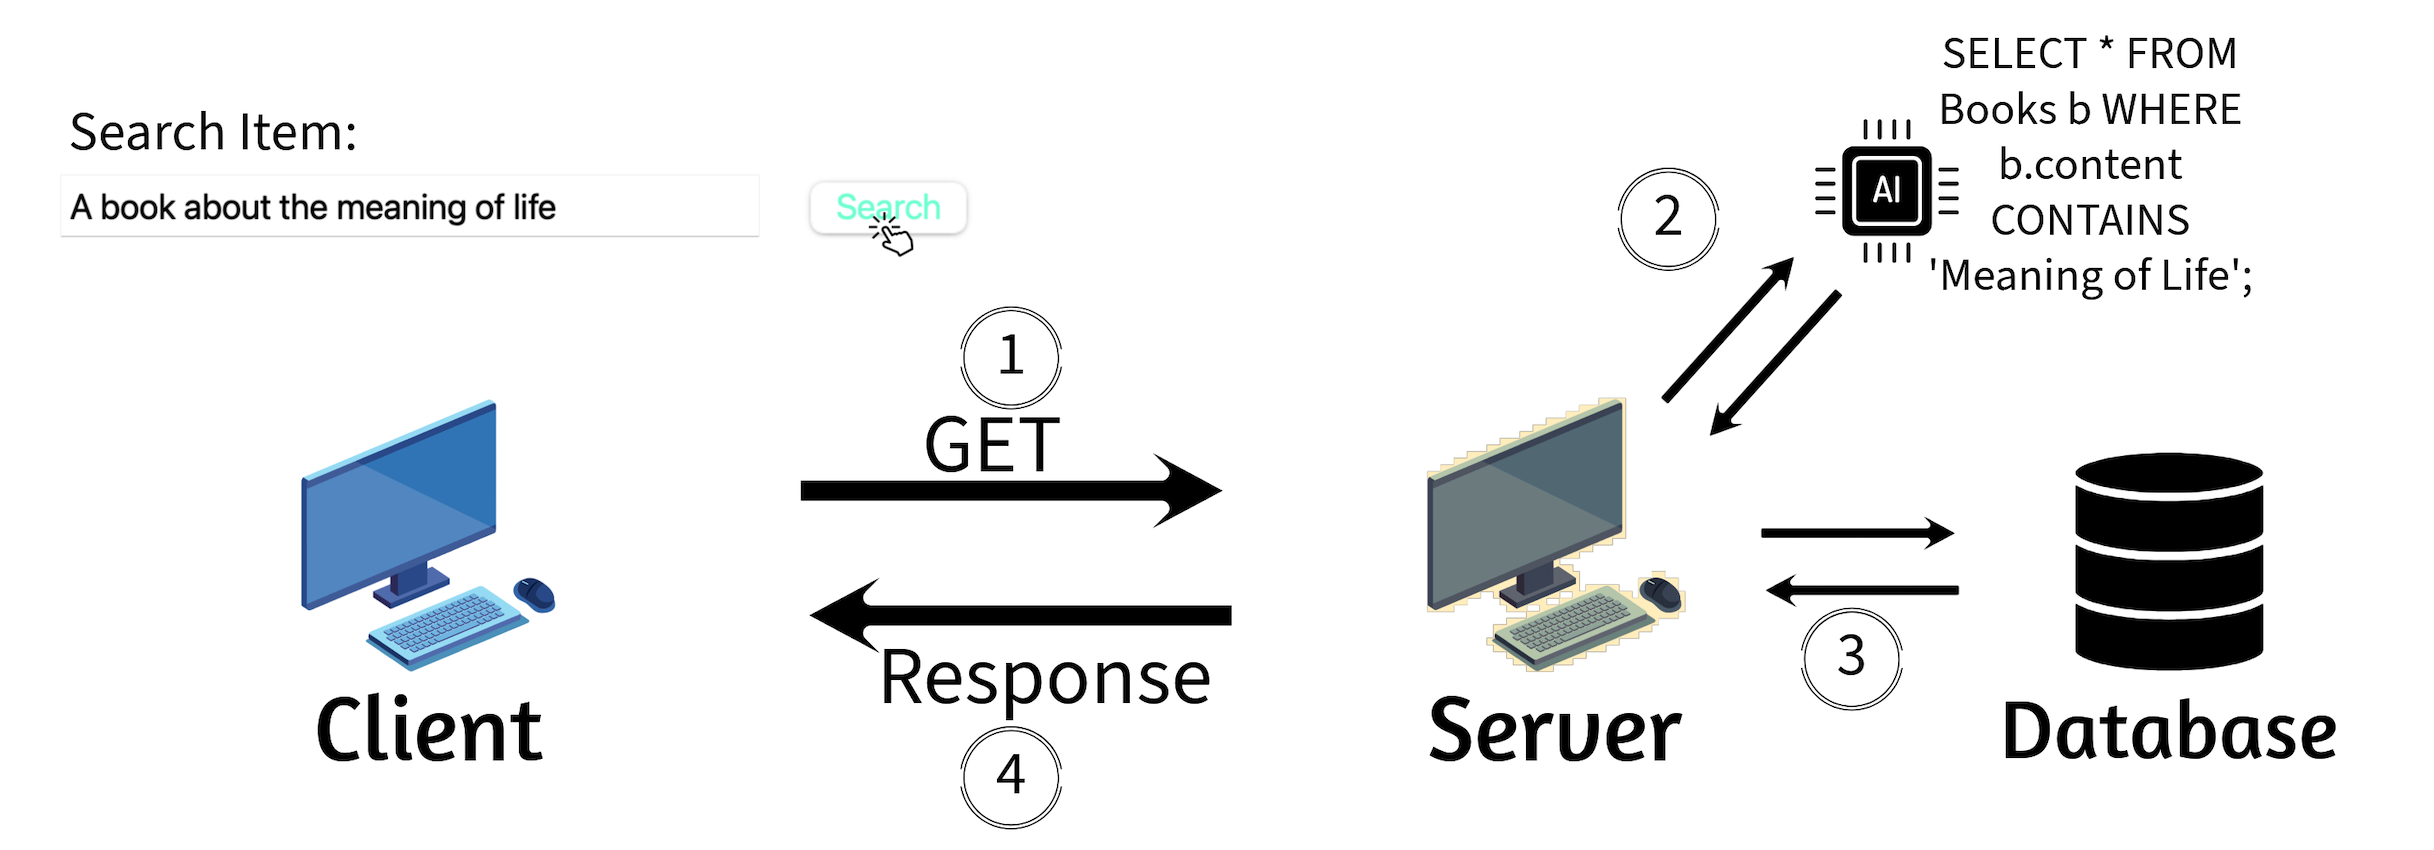
\includegraphics[width=\textwidth]{images/front_image}
  \Description{A Figure displaying the client-server interatction,
  where the input text from a user does not get concatenated
  to a static SQL-Template but is interpreted by an AI.}
  \caption{Highlighting the interaction paradigm of the user with an AI. Instead
  of traditionally passing the users input to a static SQL-Template, it is passed 
  to an AI-System that interpretes the users search request and dynamically generates a SQL-Query
  . The resulting query is then executed and displayed for the user in the Interface.}
\end{figure}

\subfile{sections/Introduction/Introduction.tex}

\subfile{sections/background/background.tex}

\subfile{sections/methods/methods.tex}


\subfile{sections/result/result.tex}

\subfile{sections/discussion/discussion.tex}

\section{Conclusion}
This study underscores the transformative potential of AI-driven NL-to-SQL systems in e-commerce search, with 
users favoring their flexibility—such as synonym recognition (Section 4)—and reporting higher satisfaction 
(mean 1.69, SD 0.48) than with static templates (mean 3.62, SD 0.51). Practical deployment is achievable through 
our proposed blacklist configuration (Section 4.3), which effectively mitigates security vulnerabilities.\\
Yet, limitations persist. The participant pool, dominated by tech-savvy computer science students with 
only one female (Section 4.1), calls for broader demographic validation. Likewise, the basic static 
template (Section 3.1) and rudimentary Claude API prompt (Section 4.3) reflect time constraints that 
hindered refinement; additional time could have yielded a more advanced prompt to boost performance further \cite{gaoTextSQLEmpoweredLarge2023}. 
Incorporating filter-interaction metrics and testing across complex domains like electronics (Section 1.2), as 
suggested in Section 5.4, would strengthen these findings. Overcoming these technical, methodological, and 
usability challenges is essential to fulfilling the vision outlined in Section 1: a seamless, intuitive search 
experience tailored to diverse user needs, poised to reshape human-computer interaction in e-commerce and beyond.

\section{Acknowledgement}
We wish to express our sincere gratitude to our lecturer, Prof. Hendrik Heuer, at the Bergische Universität Wuppertal, for 
his insightful and valuable feedback provided following our lectures and during the final presentation of our research topic.
% I try to avoid appendices
%\appendix
%\section{Appendix}

\bibliographystyle{ACM-Reference-Format}
\bibliography{references}

\end{document}
\endinput
%%
%% End of file `sample-sigconf-authordraft.tex'.
